\documentclass[letterpaper]{article}

%% Language and font encodings
\usepackage[english]{babel}
\usepackage[utf8x]{inputenc}
\usepackage[T1]{fontenc}

%% Sets page size and margins
\usepackage[letterpaper,top=3cm,bottom=2cm,left=2cm,right=2cm,marginparwidth=1.75cm]{geometry}

%% Useful packages
\usepackage{amsmath}
\usepackage{graphicx}
\usepackage[colorinlistoftodos]{todonotes}
\usepackage[colorlinks=true, allcolors=blue]{hyperref}
\usepackage{mathtools}
\usepackage{latexsym}

\title{Speech Processing Project 1 Writeup}
\author{Matt Ruffner}

\begin{document}
\maketitle

\section{}
Choosing a frame size of 512 simplified things in that I was able to use nFFT=frame size for the majority of the project. It also provided a decent (~50ms) temporal resolution. 75\% overlap was used in the spectrogram to obtain artificially high temporal resolution and decent appearance (compared to a Praat spectrogram, for example).

\section{}
Energy and zero crossing rate seem to be an excellent feature for representing the voiced/unvoiced status of a phoneme. As shown in the plots, the zero crossing rate is substantially higher for unvoiced phonemes than for voiced phonemes. Conversely, the signal energy is much higher for voiced phonemes than for unvoiced phonemes.

\stepcounter{section}
\stepcounter{section}

\section{}
There is a clear peak visible for the two voiced phonemes of the letters "u" ($\mho$) and "n" ($n$). The $f_0$ of the $\mho$ phoneme is 1582~Hz, while the peak in the cepstrum corresponding to the $f_0$ of the $n$ phoneme is at 1152~Hz.


\section{}
A cutoff of 50 was used because this was the position within the cepstra which accurately separated the vocal tract filter information from the excitation information for both of the voiced phonemes.

\section{}
I think the order 14 gives the most accurate information regarding the vocal tract filter. The 40th order filter provides an over-fitted model and the main structure of the filter is not as easily interpreted.


\stepcounter{section}
\newpage


\section{}
The formant tracks and fundamental frequency contour of the \texttt{sun.wav} audio file is shown in Fig. \ref{praat}. The red dots show the formant tracks and the blue line is the $f_0$ contour.
\begin{figure}[h!]
\centering
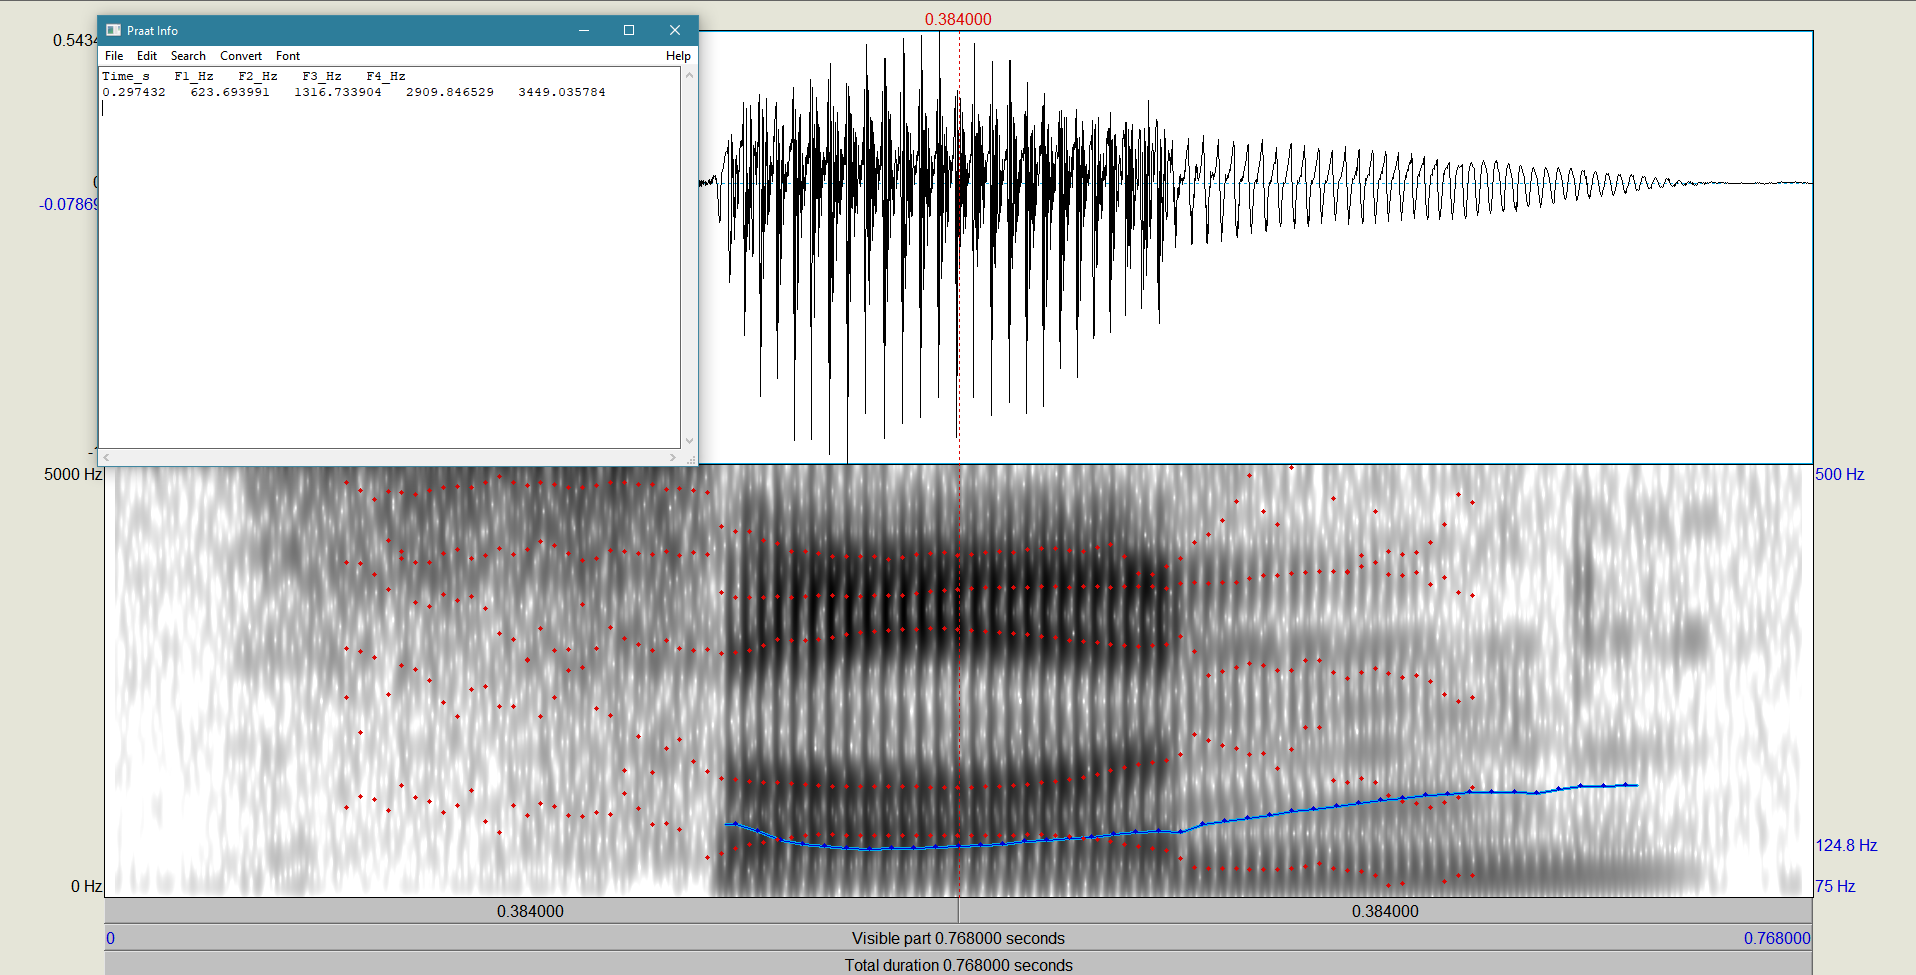
\includegraphics[width=\textwidth]{part9praat}
\caption{Spectrogram of \texttt{sun.wav} with $f_0$ contour and formant tracks.}
\label{praat}
\end{figure}


\newpage
\section{}
In this section, three tables are presented which show the formant frequencies as they are estimated from the various plots that were produced as a result of the exercises in this project. The formants in Table \ref{tab:sFormant} are for the $s$ phoneme, the formants in Table \ref{tab:uFormant} are for the $\mho$ phoneme, and the formants in Table \ref{tab:nFormant} are for the $n$ phoneme.


\begin{table}[h]
    \centering
    \begin{tabular}{c||c|c|c|c|c||c}
          & DFT & Lift. Spec. & LPC (4) & LPC (14) & LPC (40) & Praat \\
    \hline
    \hline
    $F_1$ & 429~Hz &    390~Hz   &  ?~Hz   &     &    &    \\
    $F_2$ & 1035~Hz &   605~Hz   &  ?~Hz   &     &    &    \\
    $F_3$ & 3008~Hz &   1035~Hz  &  ?~Hz   &     &    &    \\
    \end{tabular}
    \caption{Formant Frequency comparison for the $s$ phoneme.}
    \label{tab:sFormant}
\end{table}


\begin{table}[h]
    \centering
    \begin{tabular}{c||c|c|c|c|c||c}
          & DFT & Lift. Spec. & LPC (4) & LPC (14) & LPC (40) & Praat \\
    \hline
    \hline
    $F_1$ & 625~Hz  &    703~Hz    & 1465~Hz  &     &    &    \\
    $F_2$ & 1250~Hz &    1211~Hz   & ?~Hz     &     &    &    \\
    $F_3$ & 3164~Hz &    3086~Hz   & ?~Hz     &     &    &    \\
    \end{tabular}
    \caption{Formant Frequency comparison for the $\mho$ phoneme.}
    \label{tab:uFormant}
\end{table}


\begin{table}[h]
    \centering
    \begin{tabular}{c||c|c|c|c|c||c}
          & DFT & Lift. Spec. & LPC (4) & LPC (14) & LPC (40) & Praat \\   
    \hline
    \hline
    $F_1$ & 156~Hz &  137~Hz      &  391~Hz   &     &    &    \\
    $F_2$ & 957~Hz &   1016~Hz    &  ?~Hz     &     &    &    \\
    $F_3$ & 2070~Hz &  1641~Hz    &  ?~Hz     &     &    &    \\
    \end{tabular}
    \caption{Formant Frequency comparison for the $n$ phoneme.}
    \label{tab:nFormant}
\end{table}



\end{document}